\documentclass[11pt]{beamer}
\usepackage{amsmath, amsfonts, amscd, amssymb, amsthm, graphicx, tikz}
\setbeamertemplate{navigation symbols}{}

\usepackage{natbib}
\usepackage{array}
\usetheme{eaperry}

\usepackage{changepage}
\usetikzlibrary{decorations.pathreplacing}

\bibliographystyle{aer}

\title{Area Heterogeneity and the Adoption of ``Green" Building Certifications}
\author{Evan Perry}
\institute{Spellman Program}
\date{June 8, 2021}

\begin{document}


\maketitlepage


\begin{frame}{Overview}
\tableofcontents[hideallsubsections]
\end{frame}


\newsection{What is this about?}{\textit{Research Question}}


\begin{frame}{Project Focus}
\large
\begin{exampleblock}{\large\textbf{Research Question}}
What places attract energy-efficient buildings? How do neighborhood and area characteristics relate to the number of certified energy-efficient buildings?
\end{exampleblock}
\end{frame}


\newsection{Why should we care?}{\textit{Motivation}}


% This slide removed for the sake of time
%\begin{frame}{The Threat of Climate Change}
%
%\textit{``It is extremely likely that human influence has been the dominant cause of the observed warming since the mid-20th century"} \citep{ipcc2014climate}
%
%\vfill
%\begin{itemize}
%\item \href{https://www.who.int/news-room/fact-sheets/detail/climate-change-and-health}{250,000 additional deaths per year} between 2030 and 2050  \citep{WHO}
%\begin{itemize}
%	\item Heat stress
%	\item Insect-borne disease
%	\item Natural disasters, drought, famine
%\end{itemize}
%\item Depress global GDP by 2-10\% by 2100 \citep{OECD2015}
%\end{itemize}
%\end{frame}


\begin{frame}{Figure 1: Climate Change Mortalities}
\begin{center}
\href{http://www.impactlab.org/research/valuing-the-global-mortality-consequences-of-climate-change-accounting-for-adaptation-costs-and-benefits/}{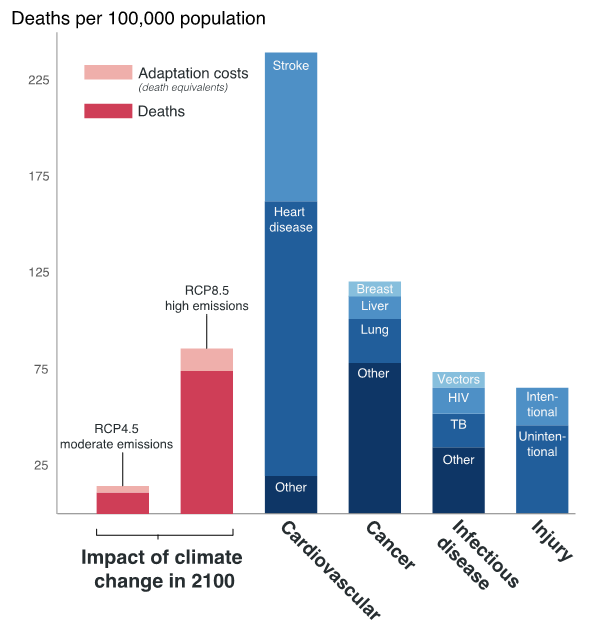
\includegraphics[scale=.85]{Figure-3.png}}
\end{center}
Credit: \cite{carleton2020valuing}
\end{frame}


\begin{frame}{Why Buildings?}
\begin{itemize}
\item 30\% of U.S. Greenhouse Gas Emissions come from Buildings (Resources for the Future, 2021)
\begin{itemize}
	\item 12\% directly at buildings
	\item 18\% indirectly from electricity
\end{itemize}
\vfill
\pause
\item Energy Efficiency is an apparent Win-Win
\vfill
\pause
\item It's timely -- the \href{https://www.whitehouse.gov/briefing-room/statements-releases/2021/03/31/fact-sheet-the-american-jobs-plan/}{American Jobs Plan} includes:
\begin{itemize}
	\item \$213 Billion to Housing
	\item More funding to the Weatherization Assitance Program
\end{itemize}
\end{itemize}
\end{frame}


\newsection{What do we already know?}{\textit{Literature Review}}


\begin{frame}{The Energy-Efficiency Gap}
\begin{definition}[Energy-Efficiency Gap]
	``The wedge between the cost-minimizing level of energy efficiency and the level actually realized." \citep{allcott2012there}
\end{definition}

\bigskip
Common Explanations \citep{gerarden2017assessing}:
\begin{itemize}
	\item Modeling Flaws
	\item Behavioral Explanations
	\item Market Inefficiencies
\end{itemize}
\end{frame}


\begin{frame}{Certifications}
Certifications can help reduce some market inefficiencies

\vspace{1.5cm}
Popular Energy-Efficient Building Certifications:
\begin{itemize}
\item Energy Star Program
\item Leadership in Energy and Environmental Design (LEED)
\item Home Energy Rating System (HERS) Index
\end{itemize}
\end{frame}


\newsection{How will we do this?}{\textit{Data \& Methodology}}


\begin{frame}{Data Sources}
\begin{itemize}
	\item LEED Project Directory
	\begin{itemize}
		\item Address, Certification Date, Building Type for mostly Commercial buildings
		\item Over 100,000 points
	\end{itemize}
	\vfill
	\item Energy Star Certified Buildings Registry
	\begin{itemize}
		\item Address, Certification Date, Building Type for Commercial buildings and Multifamily Housing
		\item Over 30,000 points
	\end{itemize}
	\vfill
	\item Create counts at the census tract level
\end{itemize}


\end{frame}


\begin{frame}{Data Structure}
\centering
\begin{tikzpicture}
	\draw[thick,rounded corners,  EAPyellow, fill = EAPyellow!30!] (-5.2,-6.7) rectangle (5.2,-1.5);
    \node[black] at (0,-2) {State/Region: Area Data e.g. Climate};
    \draw[thick,rounded corners, EAPgreen, fill = EAPgreen!30!] (-5.1,-6.6) rectangle (5.1,-3.5);
    \node[black] at (0,-4) {MSA: Area Data e.g. Utility Costs, Housing Stock};
    \draw[thick,rounded corners, EAPviolet, fill = EAPviolet!30!] (-5,-6.5) rectangle (5,-5.5);
    \node[black] at (0,-6) {Census Tract: LEED Directory, Energy Star Registry};
\end{tikzpicture}
\end{frame}


\begin{frame}{Figure 2: A Multilevel Modeling Framework}
\begin{adjustwidth}{-1cm}{-1cm}
\centering
    \begin{tikzpicture}[grow = down, scale = 1, semithick]
    \draw[thick,rounded corners,  EAPyellow,fill = EAPyellow!30!] (-5.85,-6.7) rectangle (5.85,-1.5) {};
    \draw[thick,rounded corners, EAPgreen,fill = EAPgreen!30!] (-5.75,-6.6) rectangle (5.75,-3.5) {};
    \draw[thick,rounded corners, EAPviolet,fill = EAPviolet!30!] (-5.65,-6.5) rectangle (5.65,-5.5) {};
    
    \tikzstyle{level 1}=[level distance=20mm,sibling distance=28mm]
    \tikzstyle{level 2}=[level distance=20mm,sibling distance=14mm]
    \tikzstyle{level 3}=[level distance=20mm,sibling distance=7.5mm]
        
    \tikzstyle{solid node}=[rectangle, draw, inner sep = 5, fill = white, semithick,fill opacity = 0,text opacity = 1]
    \tikzstyle{dotted node}= [inner sep = 2, fill = white,fill opacity = 0,text opacity = 1]
    \tiny
    \node[solid node]{U.S.}
        child{node[solid node]{$S_1$}
                child{node[solid node]{$MSA_{11}$}
                        child{node[solid node]{$CT_{111}$}
                                edge from parent node[]{}}
                        child{node[dotted node]{$\cdots$}
                                edge from parent node[]{}}
                        child{node[solid node]{$CT_{11\ell}$}
                                edge from parent node[]{}}
                    edge from parent node[]{}}
                child{node[dotted node]{$\cdots$} 
                    edge from parent node[]{}}
                child{node[solid node]{$MSA_{1j}$}
                        child{node[solid node]{$CT_{1j1}$}
                                edge from parent node[]{}}
                        child{node[dotted node]{$\cdots$}
                                edge from parent node[]{}}
                        child{node[solid node]{$CT_{1jm}$}
                                edge from parent node[]{}}
                    edge from parent node[]{}}             
            edge from parent node[right]{}}
        child{node[dotted node]{$\cdots$}
                edge from parent node[]{}}
        child{node[solid node]{$S_i$}
                child{node[solid node]{$MSA_{i1}$}
                        child{node[solid node]{$CT_{i11}$}
                                edge from parent node[]{}}
                        child{node[dotted node]{$\cdots$}
                                edge from parent node[]{}}
                        child{node[solid node]{$CT_{i1n}$}
                                edge from parent node[]{}}
                    edge from parent node[]{}}
                child{node[dotted node]{$\cdots$} 
                    edge from parent node[]{}}
                child{node[solid node]{$MSA_{ik}$}
                        child{node[solid node]{$CT_{ik1}$}
                                edge from parent node[]{}}
                        child{node[dotted node]{$\cdots$}                                    edge from parent node[]{}}
                        child{node[solid node]{$CT_{ikp}$}
                                edge from parent node[]{}}
                    edge from parent node[]{}}             
            edge from parent node[right]{}};
	    \draw[thick,rounded corners,  EAPyellow] (-5.85,-6.7) rectangle (5.85,-1.5) {};
        \draw[thick,rounded corners, EAPgreen] (-5.75,-6.6) rectangle (5.75,-3.5) {};
        \draw[thick,rounded corners, EAPviolet] (-5.65,-6.5) rectangle (5.65,-5.5) {};
    \end{tikzpicture}
\end{adjustwidth}
\end{frame}


\newsection{What's next?}{}


\begin{frame}{Summary}
\begin{enumerate}
	\item \textit{What is this about?}\\
	
	Characterizing the areas where there are lots of certified energy-efficient buildings
	\vfill
	\pause
	\item \textit{Why should we care?}\\
	
	Climate change threatens our world and buildings are a significant contributor
	\vfill
	\pause
	\item \textit{What do we already know?}\\
	
	There is an apparent energy-efficiency gap and certifications help close it
	\vfill
	\pause
	\item \textit{How will we do this?}\\
	
	Use data to estimate a multilevel model
\end{enumerate}
\end{frame}


\begin{frame}{Next Steps}
\textit{}
\begin{itemize}
	\item Continue the hunt for residential data
	\item Start cleaning data
	\item Read more papers:
	\begin{itemize}
			\item Investigate the theory behind the energy-efficiency gap
			\item {\bf Allcott, Hunt and Michael Greenstone}, ``Is there an energy efficiency
  gap?,'' {\it Journal of Economic Perspectives}, 2012, {\it 26} (1), 3--28.
	\end{itemize}
\end{itemize}
\end{frame}


\fakesection{Questions?}{}


\begin{frame}[allowframebreaks]{References}
\small
\bibliography{Sources}
\end{frame}

%%%%%%%%%%%%%%%%%%%%
% "Appendix"
%%%%%%%%%%%%%%%%%%%%

\begin{frame}{Figure 3: U.S. GHG Emissions by Sector}
\begin{adjustwidth}{-1cm}{-1cm}
\href{https://media.rff.org/documents/RFF-Resources-magazine-issue-207.pdf}{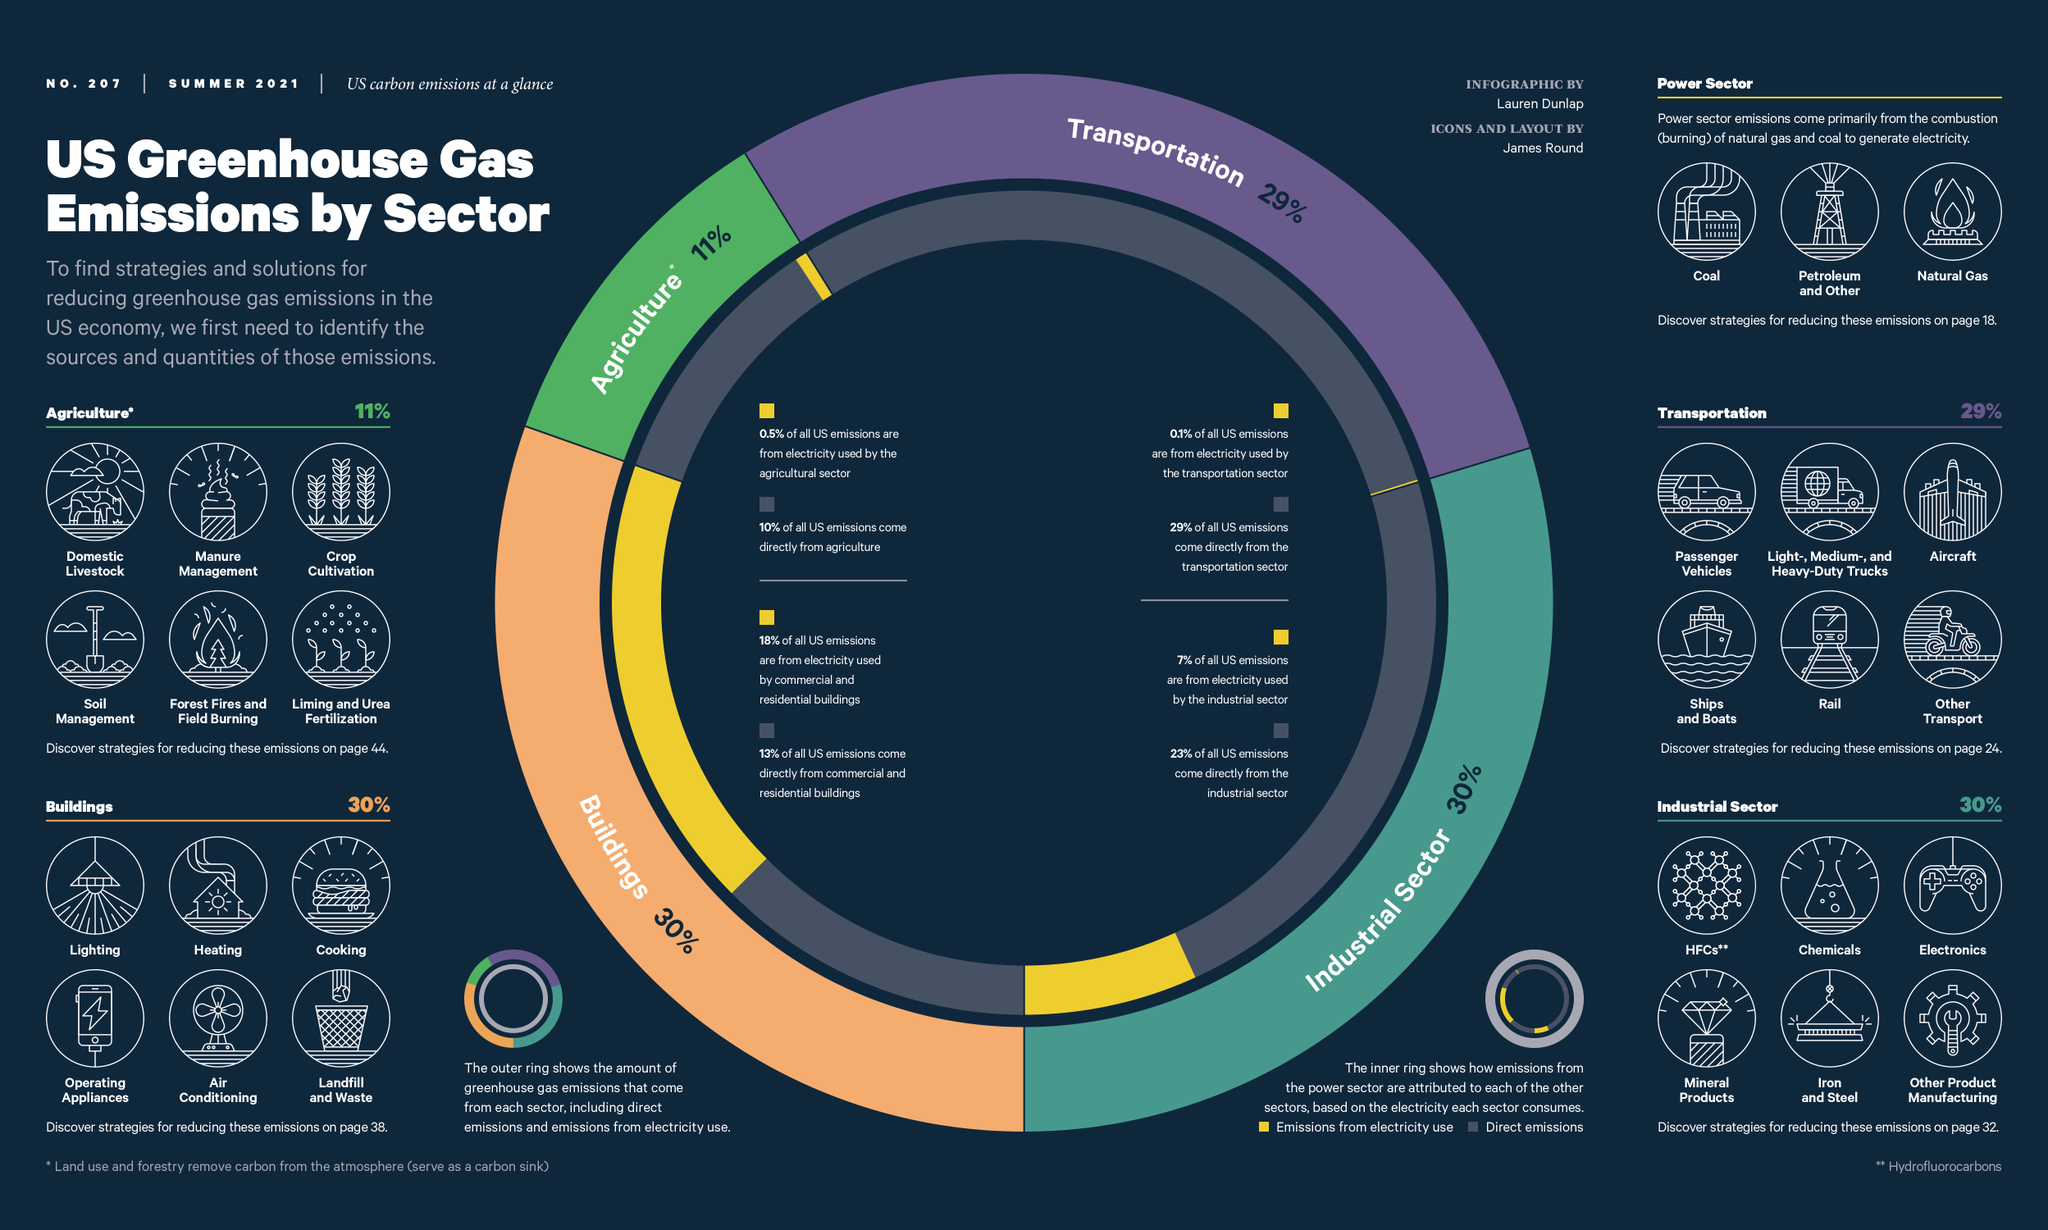
\includegraphics[width=128mm]{rff.png}}
\end{adjustwidth}
Credit: \cite{rfftoolkit}
\end{frame}


\begin{frame}{Table 1: Data Sources}
\centering
\begin{tabular}{>{\raggedright\arraybackslash}p{0.7\textwidth} >{\raggedright\arraybackslash}p{0.25\textwidth}}
\hline \hline\\ [-1.8ex]
Data Source & Data Level\\
\hline \\ [-1.8ex]
LEED Project Directory & Point \\ \\[-1.8ex]
Energy Star Certified Buildings Registry & Point  \\ \\[-1.8ex]
American Community Survey (ACS) & Census Tract \\ \\[-1.8ex]
Utility Rate Database (URDB) & Zip Code \\ \\[-1.8ex]
American Housing Survey (AHS) & MSA\\ \\[-1.8ex]
Energy Star Program Indicators & State \\ \\[-1.8ex]
Commercial Building Energy Consumption Survey (CBECS) & Regional\\
\hline \hline
\end{tabular}
\end{frame}

\end{document}